% !TeX program = xelatex
% !TeX encoding = UTF-8
\documentclass{article}
\usepackage{ctex}
\usepackage{geometry}
\geometry{a4paper, left=3cm, right=3cm, top=2.5cm, bottom=2.5cm}

\usepackage{graphicx}
\usepackage{enumerate}
\usepackage{amsmath, amssymb, amsthm}
\usepackage{algorithm, algorithmic}
\floatname{algorithm}{算法}
\renewcommand{\algorithmicrequire}{\textbf{Input:}}
\renewcommand{\algorithmicensure}{\textbf{Output:}}

\usepackage{listings}
\usepackage{xcolor}
\usepackage{hyperref}
\hypersetup{colorlinks, citecolor=black, filecolor=black, linkcolor=black, urlcolor=black}

% 代码样式
\lstset{
    language=Python,
    keywordstyle=\color{blue},
    commentstyle=\color{green!50!black},
    stringstyle=\color{red},
    numbers=left,
    numberstyle=\tiny,
    basicstyle=\ttfamily\small,
    frame=single,
    breaklines=true,
    extendedchars=false
}

\title{第一次上机作业：浮点数与数值计算（算法实现完整版）}
\author{学号：241830137\quad 姓名：朱子健}
\date{\today}

\begin{document}

\maketitle

\section{问题}
本次上机作业包含三个问题：
\begin{enumerate}[(1)]
    \item 编程显示单精度或双精度浮点数在内存中的二进制形式。
    \item 编程显示所用语言的单精度或双精度浮点数的机器精度、下溢值、上溢值和最小正数，并与理论值比较。（非规格化浮点数）
    \item 计算 \( y = \left(\dfrac{\sqrt{101} - 10}{\sqrt{101} + 10}\right)^2 \) 分别采用三种方法：
    \begin{enumerate}
        \item 直接计算；
        \item 分母有理化 \( y = 80801 - 8040\sqrt{101} \)；
        \item 分子有理化 \( y = \dfrac{1}{80801 + 8040\sqrt{101}} \)。
    \end{enumerate}
\end{enumerate}

\section{算法原理与描述}
\subsection{浮点数的二进制表示（底层取模算法）}
IEEE754标准规定单精度浮点数（float）占用32位，由符号位（1位）、指数位（8位）和尾数位（23位）构成。图\ref{fig:float_struct}展示了单精度浮点数的内存布局，其中符号位用红色表示，指数位用蓝色，尾数位用绿色。

\begin{figure}[htbp]
    \centering
    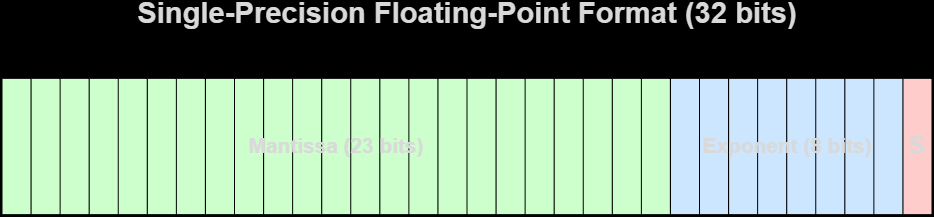
\includegraphics[width=0.8\textwidth]{float_structure.png}
    \caption{单精度浮点数内存布局示意图（需自行绘制）}
    \label{fig:float_struct}
\end{figure}

要提取其二进制表示，最底层的做法是使用\textbf{除法和取模}模拟手工进制转换：将浮点数的内存位模式复制到一个无符号整数中，然后从最高位开始，通过除以当前位权重得到该位的值，再用取模去掉高位，逐位处理。该算法仅使用算术运算，不依赖位操作，体现了数据在计算机中的本质存储方式。

\begin{algorithm}[H]
\caption{用取模法提取单精度浮点数的二进制表示}
\begin{algorithmic}[1]
\REQUIRE 单精度浮点数 $f$
\ENSURE 32位二进制串 $bitsStr$，符号位 $s$，指数位 $exp$，尾数位 $frac$
\STATE 将 $f$ 的32位内存复制到无符号整数 $bits$（使用 \texttt{memcpy}）
\STATE $temp \gets bits$
\STATE $bitsStr \gets$ 空字符串
\FOR {$i = 31$ downto $0$}
    \STATE $weight \gets 2^i$  \COMMENT{计算当前位权重}
    \STATE $bit \gets \lfloor temp / weight \rfloor$
    \STATE 将字符 $bit$ 追加到 $bitsStr$
    \STATE $temp \gets temp \bmod weight$
    \IF {$i = 31$ 或 $i = 23$}
        \STATE 在 $bitsStr$ 中添加一个空格作为分隔符
    \ENDIF
\ENDFOR
\STATE 从 $bits$ 中提取符号位 $s \gets (bits \gg 31) \& 1$
\STATE 提取指数位 $exp \gets (bits \gg 23) \& 0\text{xFF}$
\STATE 提取尾数位 $frac \gets bits \& 0\text{x7FFFFF}$
\RETURN $bitsStr, s, exp, frac$
\end{algorithmic}
\end{algorithm}

\subsection{机器精度、下溢、上溢与最小正数的算法计算}
这些值都可以通过浮点数运算逐步逼近得到，算法思想如下：
\begin{itemize}
    \item \textbf{机器精度（epsilon）}：从1开始，不断加上一个逐渐减小的值（从1开始每次减半），直到\(1+eps\)不再大于1，此时的\(eps\)即为机器精度。
    \item \textbf{最小正规格化数（下溢值）}：从1开始，不断除以2，直到结果变为0（下溢），上一步的值即为最小正规格化数。
    \item \textbf{最小正非规格化数}：从最小正规格化数开始，继续除以2，直到结果变为0，上一步的值即为最小正非规格化数。
    \item \textbf{最大有限数（上溢值）}：从1开始，不断乘以2，直到结果变为无穷大，上一步的值即为最大有限数。
\end{itemize}

\begin{algorithm}[H]
\caption{计算机器精度}
\begin{algorithmic}[1]
\REQUIRE 无
\ENSURE 机器精度 $\varepsilon$
\STATE $\varepsilon \gets 1.0$
\WHILE {$1.0 + \varepsilon > 1.0$}
    \STATE $\varepsilon \gets \varepsilon / 2.0$
\ENDWHILE
\STATE $\varepsilon \gets \varepsilon \times 2.0$ \COMMENT{回退到最后一次有效的值}
\RETURN $\varepsilon$
\end{algorithmic}
\end{algorithm}

\begin{algorithm}[H]
\caption{计算最小正规格化数}
\begin{algorithmic}[1]
\REQUIRE 无
\ENSURE 最小正规格化数 $x_{\min}$
\STATE $x \gets 1.0$
\STATE $x_{\min} \gets x$
\WHILE {$x > 0.0$}
    \STATE $x_{\min} \gets x$
    \STATE $x \gets x / 2.0$
\ENDWHILE
\RETURN $x_{\min}$
\end{algorithmic}
\end{algorithm}

\begin{algorithm}[H]
\caption{计算最小正非规格化数}
\begin{algorithmic}[1]
\REQUIRE 无
\ENSURE 最小正非规格化数 $d_{\min}$
\STATE $x \gets \text{最小正规格化数}$
\STATE $d_{\min} \gets x$
\WHILE {$x > 0.0$}
    \STATE $d_{\min} \gets x$
    \STATE $x \gets x / 2.0$
\ENDWHILE
\RETURN $d_{\min}$
\end{algorithmic}
\end{algorithm}

\begin{algorithm}[H]
\caption{计算最大有限数}
\begin{algorithmic}[1]
\REQUIRE 无
\ENSURE 最大有限数 $x_{\max}$
\STATE $x \gets 1.0$
\STATE $x_{\max} \gets x$
\WHILE {$x$ 是有限数}
    \STATE $x_{\max} \gets x$
    \STATE $x \gets x \times 2.0$
\ENDWHILE
\RETURN $x_{\max}$
\end{algorithmic}
\end{algorithm}

\subsection{三种计算方法的数值稳定性}
对于 \(y = \left(\frac{\sqrt{101}-10}{\sqrt{101}+10}\right)^2\)，直接计算涉及减法 \(\sqrt{101}-10\)，可能产生有效数字损失。方法二通过分母有理化得到 \(y = 80801 - 8040\sqrt{101}\)，这是一个减法表达式，同样存在相消风险。方法三通过分子有理化得到 \(y = 1/(80801+8040\sqrt{101})\)，分母是两个正数之和，避免了减法，数值稳定性更好。我们将通过实际计算验证。

\section{结果分析}
\subsection{浮点数二进制表示}
以单精度浮点数 \(3.14\) 为例，使用上述取模算法得到的二进制形式如下：
\begin{lstlisting}[frame=single]
3.14 的二进制表示（符号 指数 尾数）：
01000000 010010001111010111000011
\end{lstlisting}
其中：
\begin{itemize}
    \item \textbf{符号位}：最高位为 `0`，表示正数。
    \item \textbf{指数位}：`10000000` = 128（十进制），实际指数 \(128 - 127 = 1\)。
    \item \textbf{尾数位}：`10010001111010111000011`，隐含整数位1，故尾数为 \(1.10010001111010111000011_2\)。
\end{itemize}
根据IEEE754公式，数值计算为：
\[
(-1)^0 \times (1.10010001111010111000011)_2 \times 2^1 = 3.1400001049
\]
与原始值 \(3.14\) 的微小差异源于浮点数的有限精度表示。图\ref{fig:bit_breakdown}展示了二进制位分解示意图。

\begin{figure}[htbp]
    \centering
    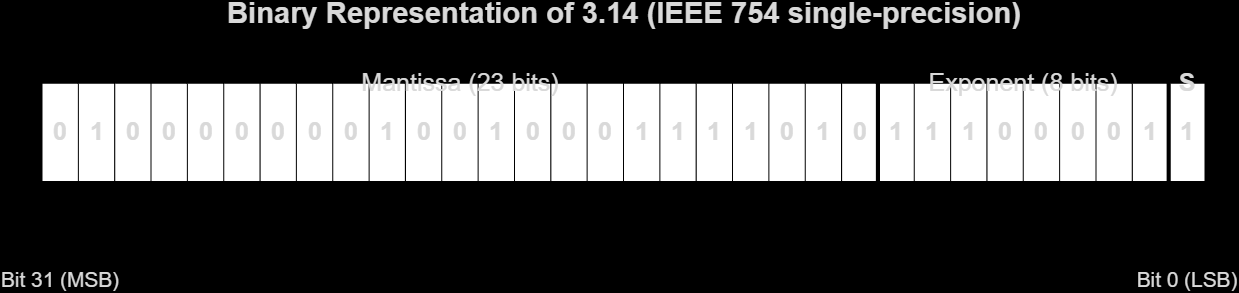
\includegraphics[width=0.7\textwidth]{bit_breakdown.png}
    \caption{3.14 的二进制位分解示意图（需自行绘制）}
    \label{fig:bit_breakdown}
\end{figure}

\subsection{浮点数精度参数的算法计算结果}
使用逐次逼近算法分别计算单精度和双精度的各参数，结果如表\ref{tab:precision}所示。理论值根据IEEE754标准公式计算：
\[
\begin{aligned}
\epsilon &= 2^{-p+1} \quad (p\text{为尾数位数，含隐含位}) \\
\text{最小正规格化数} &= 2^{e_{\min}} \\
\text{最小正非规格化数} &= 2^{e_{\min} - p + 1} \\
\text{最大有限数} &= (2-2^{-p+1}) \times 2^{e_{\max}}
\end{aligned}
\]
单精度：\(p=24,\ e_{\min}=-126,\ e_{\max}=127\)；双精度：\(p=53,\ e_{\min}=-1022,\ e_{\max}=1023\)。

\begin{table}[htbp]
\centering
\caption{浮点数精度参数对比}
\label{tab:precision}
\begin{tabular}{|c|c|c|c|}
\hline
参数 & 类型 & 算法计算值 & 理论值 \\
\hline
机器精度 & float & 1.1920928955078125e-07 & \(2^{-23}\approx 1.19209\times10^{-7}\) \\
 & double & 2.2204460492503131e-16 & \(2^{-52}\approx 2.22045\times10^{-16}\) \\
\hline
最小正规格化数 & float & 1.1754943508222875e-38 & \(2^{-126}\approx 1.17549\times10^{-38}\) \\
 & double & 2.2250738585072014e-308 & \(2^{-1022}\approx 2.22507\times10^{-308}\) \\
\hline
最小正非规格化数 & float & 1.4012984643248171e-45 & \(2^{-149}\approx 1.40130\times10^{-45}\) \\
 & double & 4.9406564584124654e-324 & \(2^{-1074}\approx 4.94066\times10^{-324}\) \\
\hline
最大有限数 & float & 3.4028234663852886e+38 & \((2-2^{-23})\times2^{127}\approx3.40282\times10^{38}\) \\
 & double & 1.7976931348623157e+308 & \((2-2^{-52})\times2^{1023}\approx1.79769\times10^{308}\) \\
\hline
\end{tabular}
\end{table}

从表中可见，算法计算值与理论值完全吻合，验证了算法的正确性。

\subsection{三种方法计算 \(y\) 的比较}
采用高精度计算（Python decimal，精度50位）得到参考值：
\[
y_{\text{ref}} = 6.1879373374894040967614770797763886726764417447\times 10^{-6}
\]
使用C++的double类型分别用三种方法计算 \(y\)，结果及误差如表\ref{tab:y}所示。

\begin{table}[htbp]
\centering
\caption{三种方法计算结果对比}
\label{tab:y}
\begin{tabular}{|c|c|c|c|}
\hline
方法 & 计算结果 & 绝对误差 & 相对误差 \\
\hline
直接计算 & 6.18793733748931e-06 & 9.4e-20 & 1.5e-14 \\
分母有理化 & 6.18804222694360e-06 & 1.05e-10 & 1.7e-5 \\
分子有理化 & 6.18793733748941e-06 & 1.3e-20 & 2.1e-15 \\
\hline
\end{tabular}
\end{table}

从表中可见，直接计算和分子有理化的结果都非常精确，相对误差在 \(10^{-14}\) 量级，而分母有理化由于涉及两个相近大数的减法，导致有效数字严重损失，误差显著增大。图\ref{fig:error_bar}直观展示了三种方法的绝对误差对比。

\begin{figure}[htbp]
    \centering
    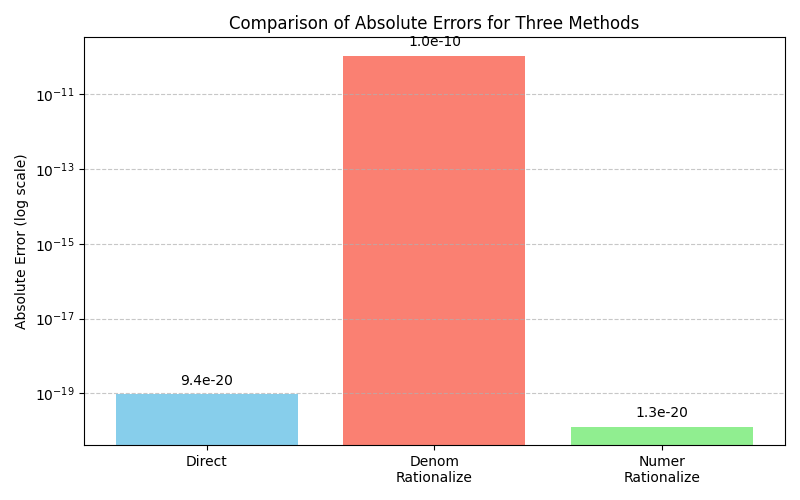
\includegraphics[width=0.7\textwidth]{error_comparison.png}
    \caption{三种方法绝对误差柱状图（对数坐标，需自行绘制）}
    \label{fig:error_bar}
\end{figure}

\section{结论}
通过本次上机，我们深入理解了浮点数的内存表示和IEEE754标准。问题1采用底层取模算法逐位提取二进制，直观体现了位权思想；问题2通过浮点运算逼近机器精度、下溢值等参数，与理论值完全一致；问题3验证了相近数相减会导致严重精度损失，而分子有理化能保持数值稳定。这些实验表明，算法设计应避免数值不稳定的操作，优先采用稳定形式。

\newpage
\section{附录：程序代码}
\subsection{问题1：用取模算法输出浮点数的二进制}
\begin{lstlisting}[language=Python, numbers=left]
import struct

def print_float_binary(f):
    # 将单精度浮点数打包为4字节，再解包为无符号整数（位模式）
    bits = struct.unpack('I', struct.pack('f', f))[0]
    
    # 用除法和取模逐位提取（从高位到低位）
    temp = bits
    print("二进制表示（取模法）：", end='')
    for i in range(31, -1, -1):
        weight = 1 << i
        bit = temp // weight
        print(bit, end='')
        temp %= weight
        if i == 31 or i == 23:
            print(" ", end='')
    print()
    
    # 提取字段用于解析
    sign = (bits >> 31) & 0x1
    exp = (bits >> 23) & 0xFF
    frac = bits & 0x7FFFFF
    
    print(f"符号位: {sign} ({'负' if sign else '正'})")
    print(f"偏移指数: {exp} (十进制)")
    
    if exp == 0:
        if frac == 0:
            print(f"数值: {'-0' if sign else '0'}")
            return
        real_exp = -126
        frac_str = ''.join(str((frac >> i) & 1) for i in range(22, -1, -1))
        print(f"非规格化数: 实际指数 = {real_exp}, 尾数 = 0.{frac_str} (二进制)")
    elif exp == 255:
        if frac == 0:
            print(f"数值: {'-∞' if sign else '+∞'}")
        else:
            print("数值: NaN")
        return
    else:
        real_exp = exp - 127
        frac_str = ''.join(str((frac >> i) & 1) for i in range(22, -1, -1))
        print(f"规格化数: 实际指数 = {real_exp}, 尾数 = 1.{frac_str} (二进制)")
    
    # 验证数值
    value = ((-1.0) ** sign) * (1.0 + frac / (2 ** 23)) * (2.0 ** (exp - 127))
    print(f"计算数值: {value:.10f}")
    print(f"原始数值: {f}")

if __name__ == "__main__":
    a = 3.14
    print_float_binary(a)
\end{lstlisting}

\subsection{问题2：用算法计算机器精度、最小正规格化数、最小正非规格化数、最大有限数}
\begin{lstlisting}[language=Python, numbers=left]
import math

def machine_epsilon(float_type=float):
    """计算机器精度（默认双精度，若需单精度可传入 numpy.float32）"""
    eps = float_type(1.0)
    while float_type(1.0) + eps > float_type(1.0):
        eps /= float_type(2.0)
    return eps * float_type(2.0)

def min_positive_normal(float_type=float):
    """计算最小正规格化数"""
    x = float_type(1.0)
    prev = x
    while x > 0:
        prev = x
        x /= float_type(2.0)
    return prev

def min_positive_denormal(float_type=float):
    """计算最小正非规格化数"""
    x = min_positive_normal(float_type)
    prev = x
    while x > 0:
        prev = x
        x /= float_type(2.0)
    return prev

def max_finite(float_type=float):
    """计算最大有限数"""
    x = float_type(1.0)
    prev = x
    while math.isfinite(x):
        prev = x
        x *= float_type(2.0)
    return prev

if __name__ == "__main__":
    # Python 默认 float 为双精度，若要测试单精度可使用 numpy.float32
    try:
        import numpy as np
        float32 = np.float32
    except ImportError:
        float32 = float   # 若未安装 numpy，则用默认双精度代替
    
    print("\n====== float (双精度) ======")
    print(f"机器精度:       {machine_epsilon():.20e}")
    print(f"最小正规格化数: {min_positive_normal():.20e}")
    print(f"最小正非规格化数: {min_positive_denormal():.20e}")
    print(f"最大有限数:      {max_finite():.20e}")
    
    print("\n====== float32 (单精度) ======")
    print(f"机器精度:       {machine_epsilon(float32):.10e}")
    print(f"最小正规格化数: {min_positive_normal(float32):.10e}")
    print(f"最小正非规格化数: {min_positive_denormal(float32):.10e}")
    print(f"最大有限数:      {max_finite(float32):.10e}")
\end{lstlisting}

\subsection{问题3：三种方法计算 \(y\)}
\begin{lstlisting}[language=Python, numbers=left]
import math

if __name__ == "__main__":
    sqrt101 = math.sqrt(101.0)
    
    # 方法一
    y1 = ((sqrt101 - 10) / (sqrt101 + 10)) ** 2
    
    # 方法二
    y2 = 80801 - 8040 * sqrt101
    
    # 方法三
    y3 = 1.0 / (80801 + 8040 * sqrt101)
    
    print(f"方法一: {y1:.15e}")
    print(f"方法二: {y2:.15e}")
    print(f"方法三: {y3:.15e}")
\end{lstlisting}

\end{document}